\chapter{Introduction}
\label{chap:intro}

\freefootnote{A reference sheet containing common notation and useful factscan be found in \cref{chap:notation}.}

Computational approaches to today's most pressing and world-changing questions are reliant on subroutines for fundamental linear algebraic tasks.
The focus of this thesis is on the design and analysis of algorithms for an increasingly prevalent subset of such tasks: those involving matrix functions of Hermitian (or real symmetric) matrices.
For the duration of this thesis, \( \vec{A} \) will be a \( n\times n \) Hermitian matrix with eigenvalues \( \Lambda := \{ \lambda_i \}_{i=0}^{n-1} \) and (orthonormal) eigenvectors \( \{ \vec{u}_i\}_{i=0}^{n-1} \); i.e.,
\begin{equation}
    \label{eqn:A}
    \vec{A} = \smop{\sum_{i=0}^{n-1}} \lambda_i \vec{u}_i \vec{u}_i^\cT.
\end{equation}
A matrix function transforms the eigenvalues of a Hermitian (or symmetric) matrix according to some scalar function, while leaving the eigenvectors untouched.
\begin{definition}
\label{def:fA}
The matrix function \( \fA \), induced by \( f:\R\to\R \) and \( \vec{A} \), is defined as 
\begin{equation*}
    \fA := \smop{\sum_{i=0}^{n-1}} f(\lambda_i) \vec{u}_i \vec{u}_i^\cT.
\end{equation*}
   
\end{definition}
Perhaps the most well known example of a matrix function is the matrix inverse \( \vec{A}^{-1} \), which corresponds to the inverse function \( f(x) = x^{-1} \). 
Other common matrix functions including the matrix sign, logarithm, exponential, square root, and inverse square root, each of which has many applications throughout the mathematical sciences.

A common task involving matrix functions is computing the product \( \fA \vec{v} \) of a matrix function \( \fA \) with a fixed vector \( \vec{v} \); for instance, the matrix inverse applied to a vector corresponds to the solution of a linear system of equations.
Beyond the multitude of applications of linear systems, matrix functions applied to vectors are used for 
computing the overlap operator in quantum chromodynamics \cite{eshof_frommer_lippert_schilling_van_der_vorst_02}, 
solving differential equations in applied math \cite{saad_92,hochbruck_lubich_97}, 
Gaussian process sampling in statistics \cite{pleiss_jankowiak_eriksson_damle_gardner_20},
principle component projection and regression in data science \cite{jin_sidford_19},
and a range of other applications \cite{higham_08}.


Another related and especially interesting task involving matrix functions is estimating the \emph{spectral sum},
\begin{equation}
    \label{eqn:spectral_sum}
    \tr(\fA) = \smop{\sum_{i=0}^{n-1}} f(\lambda_i).
\end{equation}
Applications of spectral sums include
characterizing the degree of protein folding in biology \cite{estrada_00},
studying the thermodynamics of spin systems in quantum physics and chemistry \cite{weisse_wellein_alvermann_fehske_06,schnalle_schnack_10,schnack_richter_steinigeweg_20,jin_willsch_willsch_lagemann_michielsen_deraedt_21},
benchmarking quantum devices in quantum information theory \cite{jozsa_94},
maximum likelihood estimation in statistics \cite{barry_pace_99,pace_lesage_04},
designing better public transit in urban planning \cite{bergermann_stoll_22,wang_sun_musco_bao_21}, and 
finding triangle counts and other structure in network science \cite{avron_10,dong_benson_bindel_19,benzi_boito_20}.

The trace of matrix functions is intimately related to the spectral measure of \( \vec{A} \) which encodes the eigenvalues of \( \vec{A} \).
\begin{definition}
\label{def:CESM}
The cumulative empirical spectral measure (CESM) \( \Phi : \R \to [0,1] \), induced by \( \vec{A} \), is defined by
\begin{equation*}
    \Phi(x)
    = \Phi_{\vec{A}}
    := \smop{\sum_{i=0}^{n-1}} n^{-1} \bOne[ \lambda_i \leq x].
\end{equation*}
\end{definition}
Here \( \bOne[ \texttt{true} ] =1 \) and \( \bOne[\texttt{false}] = 0 \).

Not only is \( \Phi(x) \) itself a spectral sum for each \( x\in\R \), but 
\begin{equation*}
    \tr(\fA) = n \int f\,\d\Phi.
\end{equation*}
In this sense, approximating the CESM \( \Phi \) is equivalent to approximating spectral sums.
However, approximations to \( \Phi \) are also useful in that they provide a global picture of the spectrum of \( \vec{A} \).
Such coarse grained approximations are used in 
electronic structure computations %\cite{ducastelle_cryotlackmann_70,wheeler_blumstein_72,haydock_heine_kelly_72,alben_blume_krakauer_schwartz_75,girard_87,deraedt_devries_89,skilling_89,hutchinson_89} 
and other tasks in physics\footnote{In physics, the ``density'' \( \d\Phi/\d x \) is often called the density of states (DOS).} \cite{weisse_wellein_alvermann_fehske_06,jin_willsch_willsch_lagemann_michielsen_deraedt_21},
probing the behavior of neural networks in machine learning \cite{ghorbani_krishnan_xiao_19,papyan_19,granziol_wan_garipov_19,yao_gholami_keutzer_mahoney_20}, load balancing modern parallel eigensolvers in numerical linear algebra \cite{polizzi_09,evsl_19}, and computing the product of matrix functions with vectors \cite{fan_shuman_ubaru_saad_19}.

The simplest, and arguably most elegant, approach to spectrum and spectral sum approximation involves computing quadratic forms \( \vec{v}^\cT \fA \vec{v} \) for suitably chosen random vectors \( \vec{v} \).
For any fixed \( \vec{v} \), the task of computing \( \vec{v}^\cT \fA \vec{v} \) is intimately related to quadrature \cite{golub_meurant_94,golub_meurant_09} and, besides the many applications of spectrum and spectral sum approximation, is used for estimating the error of Krylov subspace methods \cite{dahlquist_eisenstat_golub_72,golub_strakos_94,golub_meurant_09}.



%\subsection{Krylov subspace methods}
\section{Lanczos-based methods}
\label{sec:lanczos}

The algorithms we study in this thesis fall into a general class of algorithms called Krylov subspace methods (KSMs).
KSMs produce approximations using information from the set of low-degree polynomials in \( \vec{A} \) applied to a vector \( \vec{v} \); i.e. from the so-called Krylov subspace generated by \( \vec{A} \) and \( \vec{v} \).
\begin{definition}
    \label{def:Kk}
    The dimension \( k \) Krylov subspace \( \mathcal{K}_k \) generated by \( \vec{A} \) and \( \vec{v} \) is defined as
\begin{equation*}
    \mathcal{K}_{k} 
    =\mathcal{K}_{k}(\vec{A},\vec{v}) 
    := \operatorname{span}\{\vec{v}, \vec{A}\vec{v}, \ldots, \vec{A}^{k-1}\vec{v} \}
    = \{ \pA\vec{v} : \deg(p) < k \}.
\end{equation*}
\end{definition}

The information from a given Krylov subspace can be used to approximate \( \fA \vec{v} \) and \( \vec{v}^\cT \fA \vec{v} \).
In particular, a natural approach is to use the approximations 
\begin{equation*}
    \fA \vec{v} \approx  \ff{f}{s}\mf{\vec{A}} \vec{v}
    ,\qquad
    \vec{v}^\cT \fA \vec{v} \approx  \vec{v}^\cT \ff{f}{s}\mf{\vec{A}} \vec{v},
\end{equation*}
where \( \ff{f}{s} : \R\to\R \) is a degree \( s \) polynomial chosen to approximate \( f \).

Throughout this thesis, the symbol ``\( \circ \)'' should be interpreted as a parameter encompassing any other parameters which impact how \( \ff{f}{s}\mf{\vec{A}}  \) is determined for \( f \). 
For instance, once choice of \( \circ \) may correspond to the interpolating polynomial to \( f \) at some set of nodes while another choice of \( \circ \) may correspond to the Chebyshev approximation to \( f \).
Specific choices of \( \circ \) corresponding to widely used algorithms will be defined as they come up.
Here the use of ``p'' stands for polynomial, and will be used to differentiate between polynomial approximations of a function and quadrature approximations of a distribution function, which will be defined later.

\begin{remark}
When \( \vec{A} \) is Hermitian, Krylov subspace methods are, in one way or another, related to the Lanczos algorithm \cite{lanczos_50} described in \cref{alg:lanczos}.
    Even so, we use the term \emph{Lanczos-based methods} to refer to algorithms which make use of the information generated by the Lanczos algorithm in some non-trivial way. 
This is in contrast to methods, such as those based on explicit polynomial approximation, which can easily be constructed directly.
\end{remark}

\begin{assumption}
    From this point onwards, we will assume \( \|\vec{v}\|_2=1 \).
\end{assumption}


The Lanczos algorithm (\cref{alg:lanczos}) \cite{lanczos_50} produces an orthonormal basis \( \{ \vec{q}_i \}_{i=0}^{k} \) for the Krylov subspace \( \mathcal{K}_{k+1} \) such that, for all \( i = 0, 1, \ldots, k \),
\begin{equation*}
    \operatorname{span}\{ \vec{q}_0, \vec{q}_1, \ldots, \vec{q}_{i} \} = 
    \mathcal{K}_{i+1}.
%    ,\qquad \forall i\in0:k+1.%,1,\ldots, k.
\end{equation*}
These basis vectors satisfy a three term recurrence, for all \( i = 0,1, \ldots,k-1 \),
\begin{equation*}
    \vec{A} \vec{q}_i = \beta_{i-1}\vec{q}_{i-1} + \alpha_i \vec{q}_i + \beta_i \vec{q}_{i+1}
    %,\qquad \forall i \in 0:k%i = 0,1,\ldots,k-1
\end{equation*}
with initial conditions \( \vec{q}_{-1} = \vec{0} \) and \( \beta_{-1} = 0 \).
The coefficients \( \{ \alpha_i \}_{i=0}^{k-1} \) and \( \{ \beta_i \}_{i=0}^{k-1} \) defining the three term recurrence are also generated by the algorithm.
This recurrence can be written in matrix form as
\begin{equation}
    \label{eqn:lanczos_three_term}
    \vec{A} \vec{Q} = \vec{Q} \vec{T} + \beta_{k-1} \vec{q}_k \vec{e}_{k-1}^\rT
\end{equation}
where 
\begin{equation*}
    \vec{Q} := 
    \begin{bmatrix}
        |&|&&|\\
        \vec{q}_0 & \vec{q}_1 & \cdots & \vec{q}_{k-1}\\
        |&|&&|\\
    \end{bmatrix}
    ,\quad
    \vec{T} := 
    \begin{bmatrix}
        \alpha_0 & \beta_0 \\
        \beta_0 & \alpha_1 & \ddots & \phantom{\ddots}\\
        &\ddots & \ddots & \beta_{k-2} \\
        &&\beta_{k-2} & \alpha_{k-1} \\
    \end{bmatrix}.
\end{equation*}

%\begin{remark}
%Comparing the Stieltjes procedure \cref{alg:stieltjes} to the Lanczos algorithm \cref{alg:lanczos}, it is clear that they are intimately related.
%In particular, \( \vec{q}_i = p_i\mf{\vec{A}} \vec{v} \), and \( \vec{T} = \vec{M} \).
%Indeed, the Lanczos algorithm is simply the Stieltjes procedure applied to a certain weighted spectral measure which we shall discuss in the next chapter.
%\end{remark}
\begin{labelalgorithm}[H]{lanczos}{Lanczos}{Lanczos algorithm}
\begin{algorithmic}[1]
    \Procedure{\thealgorithmname}{$\vec{A}, \vec{v}, k$}
    \State \( \vec{q}_0 = \vec{v} \), \( \beta_{-1} = 0 \), \( \vec{q}_{-1} = \vec{0} \)%, \( \beta_{-1} = 0 \)
    \For {\( i=0,1,\ldots, k-1 \)}
        \State \( \tilde{\vec{q}}_{i+1} = \vec{A} \vec{q}_{i} - \beta_{i-1} \vec{q}_{i-1} \)
        \State \( \alpha_{i} = \vec{q}_i^\cT \tilde{\vec{q}}_{i+1} \)
        \State \( \hat{\vec{q}}_{i+1} = \tilde{\vec{q}}_{i+1} - \alpha_{i} \vec{q}_i \)
        \State optionally, reorthogonalize,  \( \hat{\vec{q}}_{i+1} \) against \( \{\vec{q}_j\}_{j=0}^{i} \)
        \State \( \beta_{i} = \| \hat{\vec{q}}_{i+1} \| \)
        \State \( \vec{q}_{i+1} = \hat{\vec{q}}_{i+1} / \beta_{i} \)
    \EndFor
    \State \Return \( \{ \vec{q}_i \}_{i=0}^{k} \), \( \{ \alpha_i \}_{i=0}^{k-1} \), \( \{ \beta_i \}_{i=0}^{k-1} \).
\EndProcedure
\end{algorithmic}
\end{labelalgorithm}



\begin{remark}
    It is not uncommon for the  matrices which we call \( \vec{Q} \) and \( \vec{T} \) to be denoted by \( \vec{Q}_{\mkern2mu k} \) and \( \vec{T}_k \).
    We omit these subscripts for legibility, as the number of iterations \( k \) can be treated as fixed throughout this thesis.
    Note also that we begin indexing at zero so that indices match the degree of the corresponding polynomial.
\end{remark}

%\begin{assumption}
%    Throughout this thesis, we will assume \( \|\vec{v}\|_2 = 1 \). 
%    This is essentially without loss of generality as all algorithms we discuss have an obvious dependence on  \( \| \vec{v} \| \).
%\end{assumption}

\subsection{The insufficiency of interval-based bounds}
\label{sec:poly_insuff}

As we previously noted, this thesis is concerned with polynomial approximations to \( \fA \vec{v} \) and \( \vec{v}^\cT \fA \vec{v} \).
The error of such methods is often closely related to problems in scalar polynomial approximation theory.
In particular, note that 
\begin{equation*}
    \| g \A \|_2
    = \max_{x \in \Lambda} |g(x)|
    =: \| g \|_\Lambda, 
\end{equation*}
where \( \Lambda \) is the set of eigenvalues of \( \vec{A} \).
Here we have introduced the notation \( \|g\|_S = \sup_{x \in S}|g(x)| \) for \( g:\mathbb{C}\to\mathbb{C} \) and \( S\subset \mathbb{C} \). \label{def:norm_sup}
Let \( \| \cdot \| \) be any norm induced by a positive definite matrix with the same eigenvectors as \( \vec{A} \). \label{def:norm}
Then, a simple application of the sub-multiplicative property of matrix norms (see \cref{thm:norm_exchange}) implies 
\begin{equation}
    \label{eqn:linear_form}
    \frac{\| \fA \vec{v} -  \ff{f}{s}\mf{\vec{A}} \vec{v} \|}{\|\vec{v}\|} 
    \leq \| \fA - \ff{f}{s}\mf{\vec{A}}  \|_2  
   = \| f-\ff{f}{s} \|_{\Lambda}.
\end{equation}
Recalling our assumption \( \|\vec{v}\|_2 = 1 \), we also have
\begin{equation}
    \label{eqn:quadratic_form}
    | \vec{v}^\cT \fA \vec{v} - \vec{v}^\cT \ff{f}{s}\mf{\vec{A}} \vec{v} | 
    \leq \| \fA - \ff{f}{s}\mf{\vec{A}} \|_2 \| \vec{v} \|_2^2
    = \| f-\ff{f}{s} \|_{\Lambda}.
\end{equation}
Thus, we see that the quality of our approximations can be studied in terms of the quality of the polynomial approximation \( \ff{f}{s} \) to \( f \) on the eigenvalues of \( \vec{A} \).

Since polynomial approximation on an interval is well understood, it is common to bound the quality of Krylov subspace methods in terms of the best polynomial approximations on an interval.
It is always true that 
\begin{equation*}
    \| f-p \|_{\Lambda} \leq \| f-p \|_{\mathcal{I}},
\end{equation*}
where \( \mathcal{I} := [\lmin,\lmax] \) is the smallest interval containing all of the eigenvalues.
Thus, it is common to bound the left hand sides of \cref{eqn:linear_form,eqn:quadratic_form} by an expression like
\begin{equation}
    \label{eqn:unif_bound}
    2 \min_{\deg(p) < s} \| f - p \|_{\mathcal{I}}.
\end{equation}
However, while such bounds are useful in some situations, they often provide a large overestimate of the true behavior of Lanczos-based methods and are therefore unsuitable for use as practical stopping criteria.

\subsection{The effect of finite precision arithmetic}

While reorthogonalization in the Lanczos algorithm is unnecessary in exact arithmetic, omitting it often results in drastically different behavior when using finite precision arithmetic.
Specifically, the Lanczos basis \( \vec{Q} \) may be far from orthogonal, and the tridiagonal matrix \( \vec{T} \) may be far from what would have been obtained in exact arithmetic.
Because the Lanzcos algorithm is ostensibly unstable, there has been a widespread hesitance towards Lanczos-based approaches for problems involving matrix functions, at least without reorthogonalization \cite{jaklic_prelovsek_94,silver_roeder_voter_kress_96,aichhorn_daghofer_evertz_vondelinden_03,weisse_wellein_alvermann_fehske_06,ubaru_chen_saad_17,granziol_wan_garipov_19}.

The two primary effects of finite precision arithmetic on Lanczos-based methods when run without reorthogonalization are (i) a delay of convergence (increase in the number of iterations to reach a given level of accuracy) and (ii) a reduction in the maximal attainable accuracy.
However, while both effects are easily noticeable on most problems, they do not imply that reorthogonalization is needed.
In fact, throughout this thesis, we argue that Lanczos-based methods are highly effective even without reorthogonalization.

%In fact, \emph{the first major theme of this thesis is that Lanczos-based methods for matrix functions are often the best choice of Krylov subspace methods, even when accounting for the effects of finite precision arithmetic.}

%These effects are reasonably well understood in the context of linear systems \cite{greenbaum_89,greenbaum_97a}, and for some other functions such as the matrix exponential \cite{druskin_greenbaum_knizhnerman_98}. 





\subsection{A motivating example}

We now provide a simple and familiar example chosen to illustrate the themes introduced in this section.
The conjugate gradient algorithm (CG) \cite{hestenes_stiefel_52} is used to solve positive definite linear systems of equations, and is perhaps the most well-known Lanczos-based KSM.
When applied to a positive-definite linear system \( \vec{A} \vec{x} = \vec{v} \), CG produces iterates \( \textsf{cg}_k\in\mathcal{K}_k \) optimal in the \( \vec{A} \)-norm.
This optimality implies the error bounds\footnote{Throughout, we will occasionally use symbol ``\( x \)'' for the identity function \( x: \lambda\mapsto \lambda \) rather than an unspecified real value. Thus, expressions  like \( x p \) and \( x^{-1} - p \) should respectively be interpreted to mean the functions \( \lambda\mapsto \lambda p(\lambda) \) and \( \lambda\mapsto \lambda^{-1} - p(\lambda) \).}
\begin{align}
    \frac{\| \vec{A}^{-1} \vec{v} - \textsf{cg}_k \|_{\vec{A}}}{\| \vec{v} \|_{\vec{A}}}
    &\stackrel{\text{(a)}}{\leq} \min_{\deg(p)<k} \| x^{-1} - p \|_{\Lambda} %\label{eqn:spectrum_bd}
    \stackrel{\text{(b)}}{\leq} \min_{\deg(p)<k} \| x^{-1} - p \|_{\mathcal{I}}. \label{eqn:spec_int_bd}
    %&\stackrel{\text{(a)}}{\leq} \min_{\deg(p)<k} \max_{\lambda\in\Lambda}| \lambda^{-1} - p(\lambda) | %\label{eqn:spectrum_bd}
    %\stackrel{\text{(b)}}{\leq} \min_{\deg(p)<k} \max_{\lambda\in\mathcal{I}} | \lambda^{-1} - p(\lambda) |. \label{eqn:spec_int_bd}
\end{align}

Given \( \mathcal{I} = [\lmin,\lmax] \), \href{eqn:spec_int_bd}{(\ref{eqn:spec_int_bd}b)} can be computed analytically and, roughly speaking, it decreases linearly at a rate proportional to \( (1 - 1/\sqrt{\kappa}) \). 
In other words, to reach accuracy \( \epsilon \), CG requires at most \( O(\sqrt{\kappa}\log(\epsilon^{-1})) \) iterations, where \( \kappa = \lmax / \lmin \) is the condition number of \( \vec{A} \).
This is the well known \emph{root condition number bound} for CG.
On the other hand, \href{eqn:spec_int_bd}{(\ref{eqn:spec_int_bd}a)} may be significantly better than the latter bound involving \( \mathcal{I} \) and provide a more realistic picture of the convergence of CG.
However, since \href{eqn:spec_int_bd}{(\ref{eqn:spec_int_bd}a)} depends on the spectrum of \( \vec{A} \), which is typically unknown, the bound's use is in that it provides intuition into the theoretical behavior of CG rather than as a practical stopping critera.

\begin{figure}
    \begin{center}
        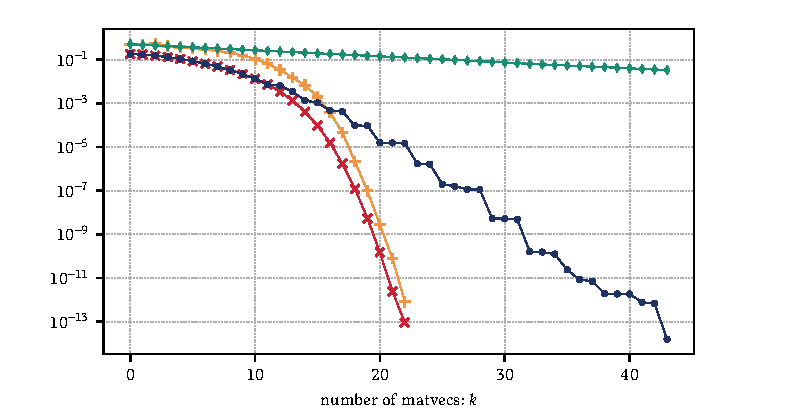
\includegraphics{imgs/ch1_unif_vs_spec.pdf} 
    \end{center}
    \caption[CG convergence (with and without reorthgonalization) and error bounds.]{%
    CG convergence (with and without reorthgonalization) and error bounds.
    \hspace{.25em}\emph{Legend}:
    CG error \( \| \vec{A}^{-1} \vec{v} - \textsf{cg}_k \|_{\vec{A}} / \| \vec{v} \|_{\vec{A}} \) with 
    ({\protect\raisebox{0mm}{\protect
\includegraphics[]{imgs/legend/l2.pdf}}}) 
    and without
    ({\protect\raisebox{0mm}{\protect
\includegraphics[]{imgs/legend/l1.pdf}}})
    reorthgonalization, 
    bound \href{eqn:spec_int_bd}{(\ref{eqn:spec_int_bd}a)} on \( \Lambda \) 
    ({\protect\raisebox{0mm}{\protect
\includegraphics[]{imgs/legend/l4.pdf}}}),
    and bound \href{eqn:spec_int_bd}{(\ref{eqn:spec_int_bd}b)} on \( \mathcal{I} \) 
    ({\protect\raisebox{0mm}{\protect
\includegraphics[]{imgs/legend/l3.pdf}}}).
    }
    \label{fig:ch1_unif_vs_spec}
\end{figure}

In \cref{fig:ch1_unif_vs_spec}, we plot the bounds \href{eqn:spec_int_bd}{(\ref{eqn:spec_int_bd}a)} and \href{eqn:spec_int_bd}{(\ref{eqn:spec_int_bd}b)} as well as the actual errors in a Lanczos-based implementation of CG run with and without reorthogonalization for a spectrum with exponentially spaced eigenvalues (the precise details are not important at this point).
Observe that the bound \href{eqn:spec_int_bd}{(\ref{eqn:spec_int_bd}a)} decreases significantly faster than \href{eqn:spec_int_bd}{(\ref{eqn:spec_int_bd}b)} for the given spectrum.
Note also that, even without reorthogonalization, CG converges significantly faster than \href{eqn:spec_int_bd}{(\ref{eqn:spec_int_bd}b)}.


An alternative to CG is the Chebyshev semi-iterative method \cite{glanders_shortley_50,gutknecht_rollin_02}.
This method can be implemented without using the Lanczos algorithm by directly constructing an explicit polynomial approximation to \( x^{-1} \) on \( \mathcal{I} \). 
However, as a result, the algorithm is unable to adapt to the spectrum of \( \vec{A} \) and usually converges very similarly to \href{eqn:spec_int_bd}{(\ref{eqn:spec_int_bd}b)}.
Moreover, if \( \mathcal{I} \) is estimated inaccurately, then the algorithm may become unstable. 
Interestingly, even in finite precision arithmetic, an iterate very close to what would be produced by the Chebyshev method can be obtained from the Lanczos method \cite{greenbaum_89,druskin_knizhnerman_91,musco_musco_sidford_18}.
Since the extreme eigenvalues of \( \vec{T} \) typically provide a very good estimate for \( \mathcal{I} \), this means that a Lanczos-based implementation of the Chebyshev method avoids the need for a priori parameter selection.

\begin{remark}
    Optimization algorithms such as accelerated gradient descent also attain a root condition number iteration complexity on any smooth and strongly convex function (such as \( \vec{x} \mapsto \frac{1}{2} \vec{x}^\cT \vec{A} \vec{x} - \vec{x}^\cT \vec{v} \) for positive definite linear systems).
Since this rate is optimal among first-order methods for smooth and strongly convex functions, accelerated gradient descent is often referred to as ``optimal''.
The fact that CG has a similar convergence guarantee often leads CG to be introduced as an alternative to accelerated gradient descent for linear systems.
However, accelerated gradient descent is essentially equivalent to the Chebyshev semi-iterative method when applied to the above objective and therefore is not typically competitive with CG in terms of the number of matrix-vector products.
\end{remark}

%\section{Some historical context}

\section{Context and contributions}
\iffalse
The Lanczos method was introduced in 1950 as a eigenvalue algorithm \cite{lanczos_50}
The conjugate gradient algorithm was also introduced in the early 1950s, and is typically attributed the joint paper of Hestenes and Stiefel \cite{hestenes_stiefel_52}, although Hestenes, Stiefel, and Lanczos \cite{lanczos_50,lanczos_52} all had earlier work involving the algorithm.
For a more comprehensive overview on the early history of the algorithms, we turn readers to \cite{golub_oleary_89}


Based on earlier works by 


National Bureau of Standards (now the National Institute of Standards and Technology).

\fi
%There are a number of books, theses, and monographs which discuss the use of Krylov subspace methods for tasks involving matrix functions.
Essentially any numerical linear algebra textbook will have at least one chapter on KSMs.
In fact, there are a number of texts which focus on the classical uses of KSMs: eigenvalue problems and solving linear systems of equations \cite{paige_71,greenbaum_97,saad_11,meurant_strakos_06,meurant_06,liesen_strakos_13}; see also \cite{golub_oleary_89} for a historical overview of early developments.
The large number of such resources means that treatments of topics such as the behavior of algorithms in finite precision arithmetic can be found at a range of levels of detail. 

Resources dealing with general matrix functions are less plentiful.
While many textbooks might have a chapter on functions such as the exponential or square root, the only recent book I am aware of which is dedicated specifically to matrix functions is \cite{higham_08}.
However, this book is focused primarily on the case of computing \( \fA \), with only one chapter devoted to the task of computing \( \fA \vec{v} \) and no discussion on the task of \( \vec{v}^\cT \fA \vec{v} \).
There are a number of more specialized texts on these topics.
The topic of \( \vec{v}^\cT \fA \vec{v} \) is covered thoroughly in \cite{golub_meurant_94,golub_meurant_09} from a theoretical quadrature perspective.
A widely used practical quadrature algorithm for estimating spectral sums and spectral densities called the kernel polynomial method is discussed in \cite{weisse_wellein_alvermann_fehske_06} but not analyzed theoretically.
The thesis \cite{schweitzer_16} discusses practical error bounds for methods for computing \( \fA\vec{v} \) for symmetric and non-symmetric \( \vec{A} \) as well as restarting techniques for non-symmetric problems, and the thesis \cite{cortinovis_22} discusses low-rank approximation of matrix functions as well as stochastic trace estimation of matrix functions.
None of the above texts discuss thoroughly the impacts of finite precision arithmetic.

During my PhD studies, it became strikingly clear that the state of knowledge surrounding Lanczos-based methods for matrix functions is fragmented.
For instance, there are several lines of work within the quantum physics literature which contain results not discovered in applied math until decades later.
Conversely, practitioners in physics, data science, and machine learning, often lack knowledge regarding the practical behavior of Lanczos-based methods in finite precision arithmetic. 
While this can be partially attributed to a lack of due-diligence in studying background material, a larger problem is that the requisite background is not easily accessible to non-specialists.
In fact, some of the most relevant work on Lanczos-based methods in finite precision arithmetic is not even well known within the numerical analysis community.


This thesis aims to fill some of the gaps in the presentation of Lanczos-based methods for matrix functions by providing a comprehensive background on the topic.
Indeed, several chapters are primarily expository, with the express goal of providing a more thorough context for the other chapters. 
%Of particular interested is a chapter on the impacts of finite precision arithmetic on Lanczos-based methods for matrix functions which we hope will serve as a useful reference going forwards. 
While there are a number of technical contributions, arguably the most significant contributions of this thesis are the following two themes:
\begin{itemize}
    \item 
        Bounds based on polynomial approximation on a single interval are insufficient to describe the true behavior of Lanczos-based methods for matrix functions. 
    Instead, one should seek bounds based on the spectrum which are able to take advantage of more fine-grained spectral structure such as gaps and outlying eigenvalues.
    \item 
        While Lanczos-based methods may behave differently in finite precision arithmetic than exact arithmetic, they still outperform Krylov subspace methods based on explicit polynomial approximations. 
        Moreover, the hyper-parameters in explicit polynomial methods can be determined effectively through the use of Lanczos-based implementations.
\end{itemize}
It is my hope that the contributions of this thesis are presented in a way which will promote understanding of and intuition for Lanczos-based methods for matrix functions outside of the numerical analysis community.



This thesis contains primarily work which appears in the following papers:

\begin{refsection}
    \nocite{
    chen_trogdon_ubaru_22,
    chen_trogdon_ubaru_21,
    chen_greenbaum_musco_musco_22a,
    chen_greenbaum_musco_musco_22b,
    }
    \printbibliography[heading=none]
\end{refsection}

Rather than stapling these papers together, I have arranged the content in accordance with my broader goals for this thesis.
In addition, a large amount of new exposition has been included in order to tie things together more cleanly and to provide additional context for non-experts.
Towards this end, many of the numerical examples from the above papers have been modified for consistency with the rest of the thesis.
The files needed to generate the figures in this thesis (as well as the thesis itself) are freely available online.


%\cite{chen_cheng_22}

%\cite{chen_hallman_22}

